\section{Adversarial Examples の定式化}
\label{sec:formulation}



\subsection{Adversarial Examples の形式的な定義}
\label{subsec:def-adv-examples}
教師あり分類問題 $f_{\text{label}}: x \rightarrow y$ を考え, モデルによる予測が $f(x) = y_{\text{true}}$ となるようなデータの組 $(x, y_{\text{true}})$ を考える\footnote{
adversarial examples は, 元々モデルの予測が正しいような入力データに摂動を加えて正しかった予測を間違えさせることを目的としているので, 出発点としてモデルによる予測が正しい予測になっている入力データのみを対象にするという意味でこのように書いている.
ただし, 実際の実験では元の予測が合っていても合っていなくてもより間違えさせるような摂動を加えて評価することも多いため, ここでの取り扱いは adversarial examples を分かりやすく定義するためのものである.
}.
adversarial examples とは, 入力 $x$ に摂動 $\omega$ を加えることによって, もともとは正しかったモデルの予測を間違ったものに変えるような入力データ $x_{\text{adv}}$ である.
%
\begin{eqnarray}
f(x + \omega) = f(x_{\text{adv}}) \neq y_{\text{true}} \ \ \text{with some constraint on} \ \omega.
\label{eq:def-adv-examples}
\end{eqnarray}
%

摂動を特徴づけるために何かしらの制限を $\omega$ に課しており, この制限は人間の目にとっては $x_{\text{adv}}$ が $y_{true}$ を正解ラベルに持つのが自然であると考えられるように付与する\footnote{
adversarial examples の大きなモチベーションの一つは, 人間の目にはある正解ラベルを持つように見える入力データが DNN モデルには異なるラベルであると予測されるデータを作成することであり, そこから DNN モデルの特徴の理解や人間との認識の理解などを深めることが期待されている.
研究によっては DNN モデルも人間も間違えるような adversarial examples を考えている \cite{elsayed2018adversarial} などもあるが, 本書ではこのような内容には踏み込まない.
}.
よく使われる制限としては $\omega$ の $l_2$ ノルムや $l_\infty$ ノルムが一定値を超えないようにするというものが挙げられる.
これらは数学的・プログラム的に扱いやすいというのが主たる理由で深淵な理由があるわけではない.
一方で, 制限として「人間の目にとって落書きに見えるような」という定量化し難いものを課す場合もあるため, 式 \ref{eq:def-adv-examples} での定式化はかなり抽象的なものとしている.
より細かい分類や具体的な手法を解説する際に, 具体的にどのような制限が課されるかを明示する.

摂動となる $\omega$ をどのように求めるかが adversarial examples を作成するための主たる要素の一つであり, のちに具体的な手法を解説する際に紹介していく.
ここでは, 最も簡単な FGSM による摂動の構成方法を例示しておく.
$\omega$ を $x$ と同じ次元を持つ摂動, $\epsilon \in \mathbb{R}$ を $x$ の各要素が取りうる値の範囲の大きさと比べて十分小さいスカラー, $J(f, x, y)$ を loss function としたとき, 以下のように loss の一階微分を用いて $x_{\text{adv}}$ を求めるのが FGSM である.
%
\begin{eqnarray}
x_{\text{adv}} = x + \omega = x + \epsilon \cdot \text{sign} ( \nabla_x J (f, x, y_{\text{true}}) ).
\label{eq:adv-fgsm}
\end{eqnarray}
%
DNN の学習で通常実施するようなパラメタの微分ではなく, データの微分 $\nabla_x$ であることに注意されたい.
これは, adversarial examples の作成においては更新するのはモデルのパラメタではなくて入力データとなるためである.
この微分で入力データと同じ $m$ 次元のベクトルが得られ, その符号を取っているので, 各要素において一階微分の意味で loss function が増大する方向を取得している\footnote{
モデル学習のためによく使うパラメタの更新は $\eta > 0$ を用いて $\theta_{\text{updated}} = \theta - \eta \nabla_\theta J$ というものだったことを思い出すと, 第二項の符号が逆であり, パラメタの更新の場合は loss を小さくする方向に, adversarial examples の場合は loss を大きくする方向に動かしていることが理解できる.
FGSM に関しては \ref{subsec:fgsm-based} 節で改めて解説する.
}.
あとは摂動の大きさを調節するために $\epsilon$ を乗じているだけで, シンプルな構成方法となっていることが理解できる.

データが 2 次元の簡単な場合で図示したのが図 \ref{fig:fgsm-loss} である.
あるデータ $x$ における微分 $\nabla_x J$ を計算し, その $\text{sign}$ を取ることで $x_1, x_2$ 成分それぞれに対して正負どちらの方向に動かせば loss が大きくなるかということが分かる (図の場合はどちらも正の方向).
あとはそれに $\epsilon$ という単一の微少量を掛けて $x$ に足すことで loss が大きくなるような $x_{\text{adv}}$ を構築している.
この例では 2 次元であるので $\epsilon$ が小さいため loss の増大分は大したことはないが, これが 10,000 次元など大きくなってくると小さな $\epsilon$ が積み重なって大きな loss の増大に繋がり, その結果モデルの logit は clean なデータの場合とはかけ離れたものになり, $y_{\text{true}}$ とは異なるラベルと予測するようになる.
%
\begin{figure}[htbp]
\begin{center}
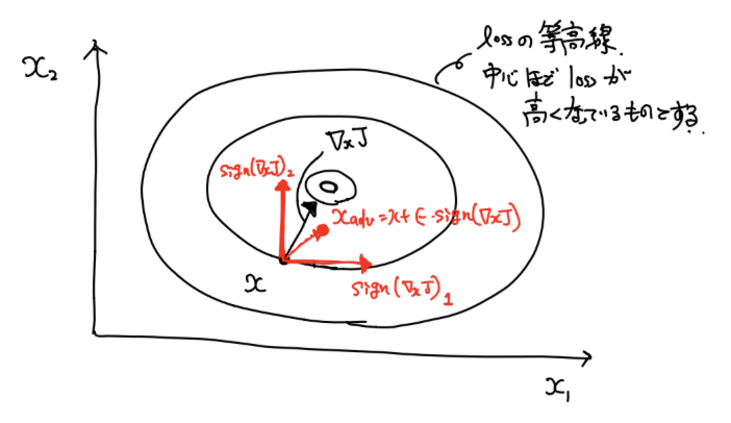
\includegraphics[width=12.0cm]{figures/fgsm-loss.pdf}
\end{center}
\caption{
FGSM による adversarial examples 作成のイメージ図.
データが 2 次元 $(x_1, x_2)$ の場合で, 黒い等高線が loss の等高線を表していて, 中心ほど loss が高くなっているものとする.
あるデータ $x$ における微分とそれに基づいて $x_{\text{adv}}$ を作る様子を示している.
}
\label{fig:fgsm-loss}
\end{figure}
%



\subsection{Adversarial Examples を用いた攻撃とそれに対する防御}
\label{subsec:attack-and-defense}
前節で定義した adversarial examples を用いて, DNN による分類をサブシステムとして含むシステムに攻撃が可能となる.
ここで言う攻撃とは, 攻撃者が adversarial examples を用いて DNN モデルの予測を誤った予測に変えることで, システムの利用者が不利益を被るものである.

具体的な例として自動運転システムのサブシステムとして車載搭載カメラで標識を画像認識する場合を考える.
システムが adversarial examples を用いた攻撃を受けた場合\footnote{
前節で紹介した FGSM は攻撃対象のモデルの微分を必要とするもので, モデルの微分情報が取得できないケースでは使用できないものである.
しかし, のちに紹介するように adversarial examples を構築する際には必ずしもモデルの情報は取得できる必要はないため, このような攻撃は現実に生じ得るものである.
}, 一旦停止の標識がある場所で一旦停止の標識と認識して止まるべき状況で速度制限の標識と誤認識することで止まらずに進んでしまい, 大事故に繋がる可能性がある.
画像認識モデルの大きな応用の一つが自動運転における人や標識などの物体認識であり, モデルの誤認識が引き起こす影響も大きいため, adversarial examples の研究でもよく題材となる.
現時点での研究でも, adversarial examples となり得る標識を実際に設置し\footnote{どのようにこれを実現するかはのちに具体的な例で紹介するが, 標識に摂動をプリントしたシールを貼ったりすることで adversarial examples を作成することが可能である.}, 車載カメラで撮影した画像がモデルに誤認識を引き起こすかを調べたりするところまで来ているため, 近い将来に実用面でも重要となる可能性を十分に秘めている.

別の例として顔認識システムのサブシステムとしてカメラで人物を特定する場合を考える.
顔認識で人物を特定して支払情報と紐づけて物品購入の支払いをする場合, adversarial examples を用いた攻撃によって実際に物品を購入した人物とは別の人物が支払いを要求される可能性がある.
また, 人物検出を実施するモデルに対して攻撃を加えて人間がいないと誤認識させることで, システムには人間が存在することを悟られることなく行動することができるかもしれない.

ここで挙げた例は極端に単純化した場合で実際のシステムはもっと頑健に作られているべきであるが, DNN に対する adversarial examples 自体は DNN 以外のシステムの頑健性とは独立に厳然として存在するものであり, 品質が保証されているべきシステムを実運用する際には脅威となり得るものである.

このような攻撃が存在する以上, 如何にして防御をしてシステムを頑健にするかが重要になる.
防御方法として, 摂動が加えられた入力データ $x_{\text{adv}}$ に対しても正しいラベル $y_{\text{true}}$ を返すようなモデルを構築する方法と,  $x_{\text{adv}}$ が adversarial examples であることを検出\footnote{
本来のモデルの予測とは別に何かしらの機構で入力データが正常なデータか adversarial examples かを二値分類する.
}してそれをシステム利用者に知らせる方法と, のようにこれらのアプローチを別の手法と分類する文献もあるが, 本書ではこれらを細かく分けずに防御方法という一つの枠内で取り扱うものとする.

攻撃側は adversarial examples による攻撃だけを考えればよく, adversarial examples の作成に多大なコスト (人的コストや時間的コストや計算資源的コスト)が掛かったとしても一度でも成功すれば被攻撃者に大きな損害を与え得る.
一方で防御側はそもそものモデルの予測が本来使いたいものなので, adversarial examples に対してはあまりコストを掛けずに対応したいというモチベーションがある.
adversarial examples に対する防御性能は高くても, モデル設計を一からやり直す必要があったり, 推論の速度が何倍にもなってしまったりするのはコストが高すぎるという状況も多いだろう.
また, 本来の目的である予測が degradation\footnote{ここでは adversarial examples に対応するようにモデルをアップデートしたときに, clean なデータに対するモデルの予測精度が低下することを指す.} を起こしてしまうのも避けたい.
さらに, 防御側は攻撃側の手法のアップデートに対応してシステムを逐次改善してアップデートしていく必要もあるため, コストの観点は重要となる.
現状の研究ではこの観点はそれほど重視されていないよう見受けられるが間違いなく重要であり, 本書では最初の一歩として定性的なコストの評価を試みている.

重要なことは, 攻撃と防御は表裏一体であり, どんなモデルに対してもうまくいく攻撃やその逆のどんな adversarial examples に対してもうまく防御できる手法は存在しないということである.
攻撃も防御も様々な手法が提案されており, それは今後も続くものであるため, 常に新しい手法を理解して取り入れていく必要がある.

次節以降では 2019 年末時点での攻撃と防御のそれぞれの典型的な手法を概念的に分類して整理し, 次章以降でそれらの詳細を解説していく.



\subsection{Adversarial Examples を用いた攻撃の分類}
\label{subsec:classification-attack}
モデルを誤認識させるための adversarial examples を作成する際の作成方法を分類する.
\cite{yuan2019adversarial} や \cite{wiyatno2019adversarial} のような adversarial examples に関するレビュー論文においても様々な軸で分類がなされているが, 統一的な分類方法は定まっていないように思われる.
本書では, 先行研究を踏まえつつ, 著者が特に重要と考える以下の観点を用いて手法を分類する.
A $\lor$ B の項目は対象の攻撃手法が A か B のどちらかに分類されることを意味している.
%
\begin{itemize}
  \item Digital (Pixel) attack $\lor$ Physical attack\\
  前者は画像のピクセルデータを直接変更して攻撃するもので, 後者は電子データではなく物理的環境で撮影する場合に対象物に物理的変更を加えて攻撃する.
  digital attack はモデルの性能を深く理解するために重要であり, また画像認識 API への攻撃などにも用いられる.
  physical attack は自動運転など物理的環境で稼働するシステムへの攻撃に用いられる.
  \item Classifier $\lor$ Detector\\
  前者は入力データに対してラベルを返すもので, 後者は入力データに対して複数の bbox の位置情報と各 bbox に対するクラス予測を返すものとする.
  adversarial examples の研究は classifier を対象とするものが多いが, 実運用では detector にも有効であるかの観点も重要であり, detector を対象とする研究も増えてきている.
  \item 摂動作成時に使用するデータ\\
  adversarial examples を作成する際にどのようなデータを使用するかという観点.
  単純なものとしては攻撃対象データを用いてそこに摂動を加えるというものが挙げられるが, モデルの構造だけに注目してデータを必要としない手法や, renderer を介する手法で 3D object データを用いるものなど多様な発展がある.
  \item 画像全体への摂動 $\lor$ 対象物のみへの摂動\\
  前者は画像の任意の点でのピクセル値を変えるもので, 後者は例えばある標識を誤認識させたい場合に対象物である標識のみに摂動を付与するものである.
  基本的に前者が digital attack で後者が physical attack である\footnote{
  もし入力データが時間不変なものであれば画像全体を対象として摂動を構築した方が攻撃成功率が高まるが, physical attack では時事刻々とシステムへ入力される画像が変わるため, 対象物以外に摂動を加えても距離や角度の変化によって誤認識を引き起こすことのできないものとなりがちである.
  physical attack では対象物のみに摂動を加え, その摂動を含む対象物がどのように撮影されようとも誤認識させるようにする必要がある.
  }
  が, digital attack でも対象物のみに摂動を付与する工夫をしてその後の physical attack につなげようとする手法も存在する.
  \item 知覚しづらさの定義\\
  作成した adversarial examples がどのような意味で「摂動」になっているかという観点.
  単純なものとしては摂動の $l_2$ ノルムが上から押さえられているというような定量的な指標が用いられ, これは元画像からの差分の評価に使えるしこの指標が小さいほど人間の目にとっても元画像と区別がつきにくい.
  発展的な指標として, 落書きのように見える (ので人間にとって特殊なノイズだと気付きにくい) という定量化が難しいものや色味が変わるだけ (なのでピクセル値の意味では変化が大きくても人間にとっては特殊なノイズだと気付きにくい) というもの, などもある.
  \item White box $\lor$ Black box\\
  前者はモデルの情報 (アーキテクチャや loss やその微分) を使ってモデルの誤認識率を高めるための手法である.
  後者はモデルの入出力のみにアクセスできる.
  実際の攻撃では black box の場合がほとんどであるが, white box は最悪ケースの想定やモデルの構造の理解, black box attack を構築するための材料として使用するなどの用途がある.
  なお, 真の black box とは出力として出力されたラベルのみを使用できるものであるべきだが, 現状は多くの提案手法で出力の全クラスに対応する softmax 値を使用している\footnote{
  $C$ クラス分類問題において, $C$ 次元の softmax 値を全て使用しているという意味.
  例えば商用の画像認識 API などは確率値の高い上位 $N (< C)$ 件のラベルしか返さないものが多く, このような設定は非現実的である.
  真の black box attack を実現している手法として \cite{tsuzuku2019structural} などが挙げられる.
  }.
\end{itemize}
%

ここで取り上げていないが典型的な観点として, Targeted / Non-targeted という, 特定のラベルに誤認識させるか正解のラベル以外なら何でもよいかというものがある.
これは前述のような真の black box attack では non-targeted しか選べないことと, targeted の多くの手法は non-targeted として使うこともできるという理由から除外している.

ここまで挙げたのは個別の手法の分類のための観点だが, 実運用上では攻撃者がどの情報にアクセスできるかが重要な観点である.
例えば画像認識 API への攻撃ならば digital attack となり, 自動運転システムの画像認識サブシステムへの攻撃ならば physical attack となる.
攻撃側としては現実的には black box attack を採用するしかないが, 防御側としてはモデルの振る舞いを理解しておくためにも white box attack を把握しておくことは不可欠である.
実運用上の観点から攻撃方法を分類したものが以下の図 \ref{fig:attack-summary} である.
例で挙げているのは \href{https://arxiv.org}{https://arxiv.org} の論文であり, 数字は arXiv の投稿番号である.
投稿番号は [YYMM.xxxxx] という形式で与えられており, 出版年の下 2 桁と月が最初の 4 文字で, 以降の数字は出版順に振られるようになっている.
本書では対象とする論文が arXiv にある場合はそれを参照するようにし, 投稿番号を併せて記載するようにする.
%
\begin{figure}[htbp]
\begin{center}
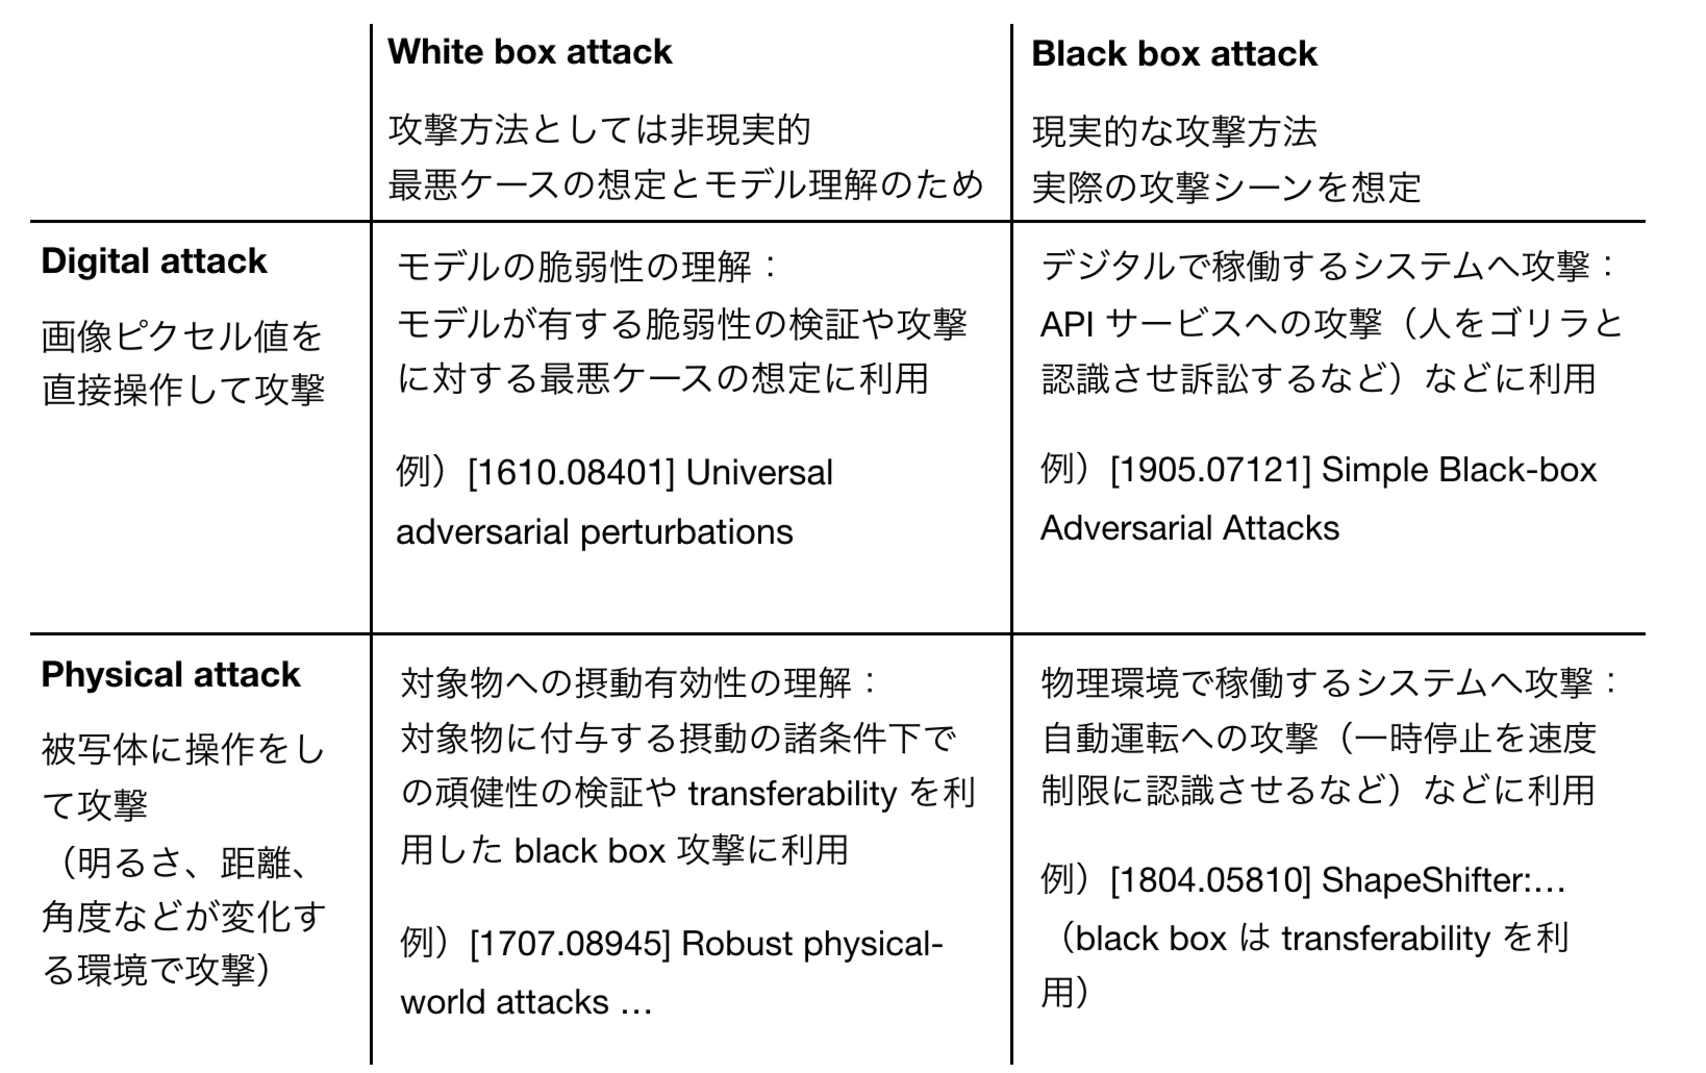
\includegraphics[width=15.0cm]{figures/attack-summary.pdf}
\end{center}
\caption{実運用上の観点に基づく攻撃方法の分類. 例は arXiv の論文であり, 投稿番号とタイトル (の一部) を記載している.}
\label{fig:attack-summary}
\end{figure}
%



\subsection{Adversarial Examples に対する防御の分類}
\label{subsec:classification-defense}
adversarial examples に対する防御手法を分類する.
攻撃方法と同様に著者が重要と考える観点で分類をするが, 他ではあまり見られない独自の観点が多いことに注意されたい.
本書の特徴として, 研究ではあまり取り上げられないが実運用上問題となる観点である「当該手法を導入するための対応コスト」という観点を含めている.
%
\begin{itemize}
  \item 基本戦略\\
  防御のための大まかな戦略を次の 4 つから成るものとした: 正則化 (学習時の loss function に正則化項を加える), 入力データ変更 (予測対象となる入力データを加工する), 予測モデル変更 (本来の予測モデルのアーキテクチャに手を加える), 外部モデル使用 (予測モデル以外のモデルを使用する).\\
  これらの分類を防御方法の分類とすることが多いと思われるが, 本書ではコストの観点を重視して分類の観点として取り入れているので, ある程度粒度を合わせるためにこれらの細かい分類をまとめて基本戦略として一つの観点にしている.
  \item 使用する外部リソース\\
  予測モデルの構築には予測モデルのアーキテクチャと学習データを準備すればよいが, 防御手法によっては更なるリソースを必要とするものも多い.
  予測モデルとは別のモデルや外部のデータ, そして防御手法のための adversarial examples\footnote{
  これは予測モデルと学習データがあれば作成できるものであるが, 便宜上外部リソースとして扱うことにする.
  } などが対象となる外部リソースである.
  \item 対応コスト (人的コスト, 推論コスト)\\
  当該の防御手法を導入するためにどれくらいのコストを必要とするかという観点.
  ここでは 2 種類のコストを考えおり, 人的コストはリソースの準備やコーディングの量や学習の待ち時間を想定しており, 推論コストは予測時に本来の予測モデルによる予測と比べて余分に必要となる計算量を想定している.
  実運用上重要だが定量化が難しい観点であるため, 大・中・小の大まかな 3 段階で評価する. 
\end{itemize}
%

繰り返しとなるが, 防御方法において重要なのはその方法を導入する際のコストがどの程度で, 実運用のプロセスに組み込むことが可能なのか, という点である.
この点を明確にすべく, モデル設計から予測までのプロセスを分解し, 防御方法がプロセスのどの段階にマッピングされるかをまとめたものが以下の図 \ref{fig:defense-process} である.
%
\begin{figure}[htbp]
\begin{center}
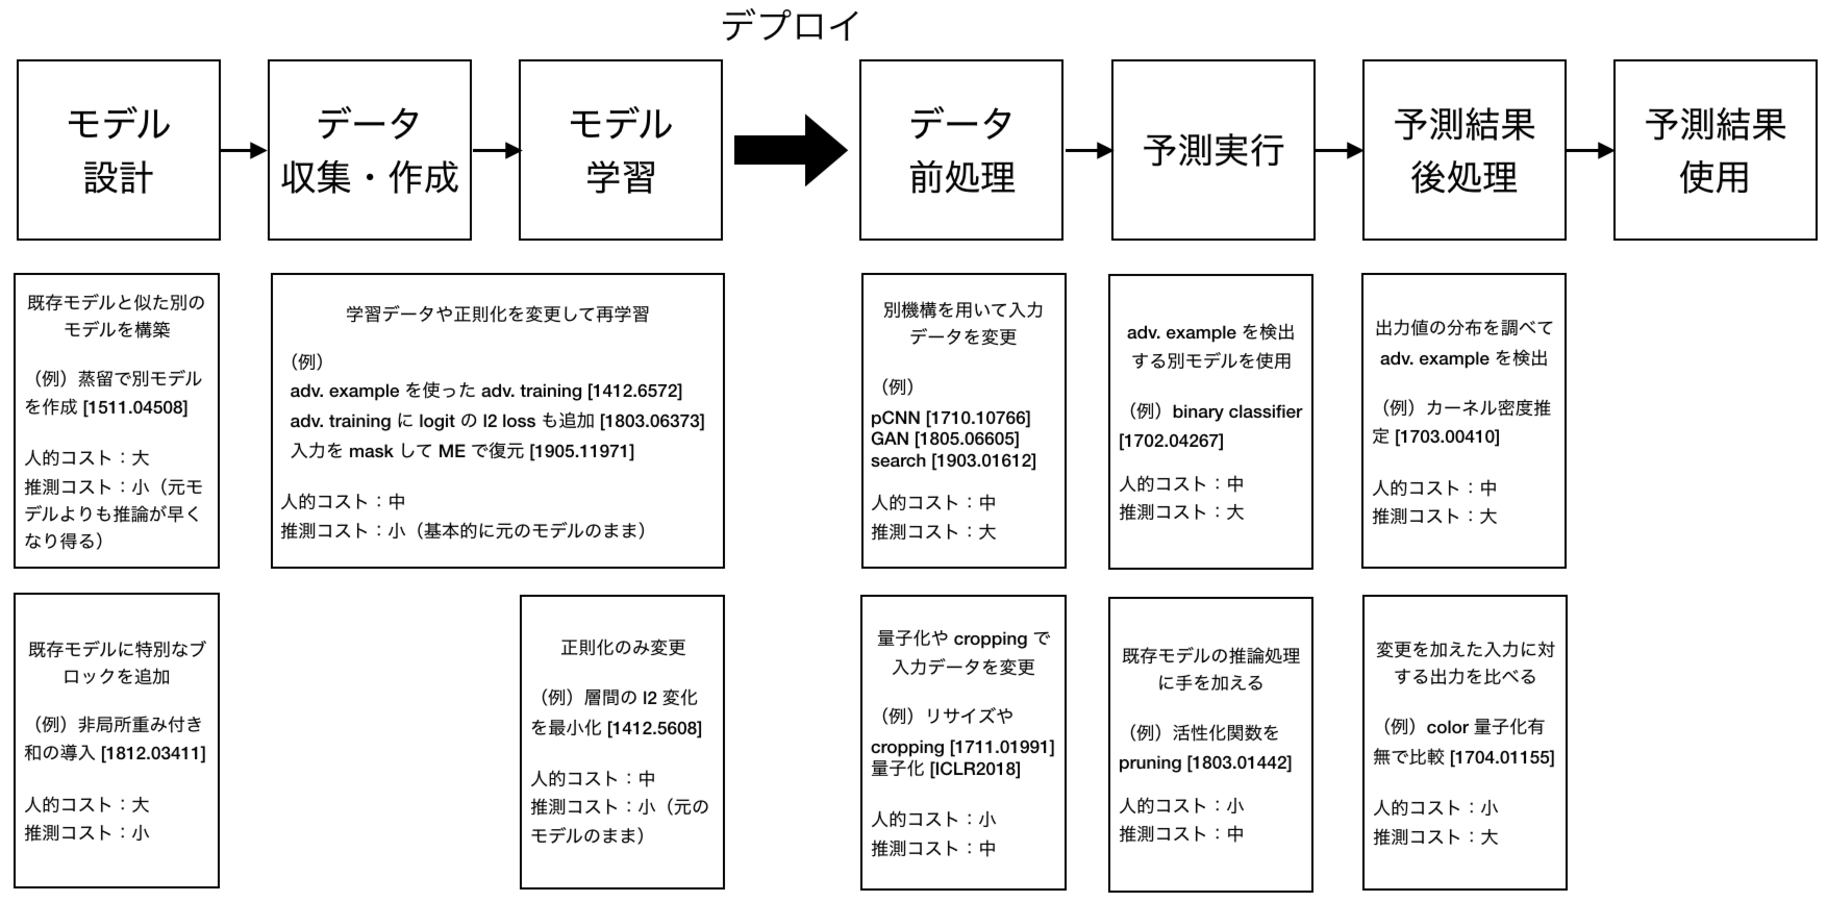
\includegraphics[width=16.0cm]{figures/defense-process.pdf}
\end{center}
\caption{
防御方法のプロセスへのマッピング.
それぞれの枠が同じ種類の防御方法を表しており, 簡単な説明と具体的な論文の例, 対応コストを記載している.
このコストは該当する枠の大まかな目安に過ぎず, 個別の手法毎に差があるため詳しくは個別の手法を見るように注意されたい.
文字が小さいため拡大して見ることを推奨.
}
\label{fig:defense-process}
\end{figure}
%